% Autor: Pablo Baeyens (@pbaeyens)
% Email: pbaeyens31+github@gmail.com
% Licencia: CC BY-SA 3.0

%% Paquetes y configuración %

% Beamer
\PassOptionsToPackage{unicode}{hyperref}  % Evita errores con caracteres no ASCII
\PassOptionsToPackage{naturalnames}{hyperref} % tex.stackexchange.com/questions/10555
\documentclass[compress]{beamer}

% Idioma
\usepackage[spanish]{babel} % Traducciones
\usepackage[utf8]{inputenc} % Uso de caracteres UTF-8
\usepackage{lmodern}        % Fuentes de tamaño arbitrario
\usepackage[T1]{fontenc}    % Permite copiar y evita errores
\uselanguage{Spanish}       % Traducciones beamer
\languagepath{Spanish}      % (tex.stackexchange.com/questions/168208)

\usepackage{multicol}
\usepackage{multirow}

% Matemáticas
\usepackage{amsfonts}
\usepackage{amsmath}
\usepackage{amssymb}
\usepackage{marginnote}
% Colores
\definecolor{backg}{HTML}{F2F2F2}    % Fondo
\definecolor{title}{HTML}{bdc3d1}    % Títulos
\definecolor{comments}{HTML}{BDBDBD} % Comentarios
\definecolor{keywords}{HTML}{08388c} % Palabras clave
\definecolor{strings}{HTML}{FA5858}  % Strings
\definecolor{links}{HTML}{2C2C95}    % Enlaces
\definecolor{bars}{HTML}{045FB4}     % Barras (gráfico)

% Código
\usepackage{listings}
\lstset{
language=[LaTeX]TeX,
basicstyle=\footnotesize,
morekeywords={href,uselanguage,languagepath,column},
otherkeywords={pause,usetheme,usecolortheme,useinnertheme,titlepage,tableofcontents,subtitle},
breaklines=true,
backgroundcolor=\color{backg},
keywordstyle=\color{keywords},
commentstyle=\color{comments},
stringstyle=\color{strings},
tabsize=2,
% Acentos, ñ, ¿, ¡ (tex.stackexchange.com/questions/24528)
extendedchars=true,
literate={á}{{\'a}}1 {é}{{\'e}}1 {í}{{\'i}}1 {ó}{{\'o}}1
         {ú}{{\'u}}1 {ñ}{{\~n}}1 {¡}{{\textexclamdown}}1
         {¿}{{?`}}1
}

% Gráficos
\usepackage{pgfplots}
\pgfplotsset{width=7cm,compat=1.8} % Opciones para gráficos

% Emoticonos
\usepackage{wasysym}
\usepackage{graphicx}
% tikz
\usepackage{tikz}
\usetikzlibrary{mindmap,trees,shadows}
\tikzset{ % Genera overlays
    invisible/.style={opacity=0},
    visible on/.style={alt={#1{}{invisible}}},
    alt/.code args={<#1>#2#3}{\alt<#1>{\pgfkeysalso{#2}}{\pgfkeysalso{#3}}},
}

%% Comandos %%
\newcommand{\ejemplo}[1]{\lstinputlisting{./examples/#1}} % Mostrar código de ejemplos
\newcommand{\muestra}[1]{\input{./examples/#1}}           % Mostrar ejemplos
\newcommand{\seccion}[1]{\input{./sections/#1}}           % Incluir secciones
\newcommand{\espacio}{\vspace*{\baselineskip}}            % Añade espacios
\newcommand{\beamer}{\texttt{beamer} }                    % Estilo único para beamer
\newcommand{\enlace}[3]{\href{#1}{\textbf{#2}} - {\small #3}}  % Estílo único para refs
\newcommand{\comando}[1]{{\color{black}\textbackslash}{\color{keywords}#1}}
\newcommand{\marginalnote}[1]{\mbox{}\marginpar{\raggedright\hspace{0pt}#1}}
%% Temas %%
% Tema y tema de color
  \usetheme{Dresden}
  \usecolortheme{dolphin}
  \useinnertheme{circles}
  \setbeamercovered{transparent}
% Colores bloques
  \setbeamercolor{block title}{bg=title,fg=links}
  \setbeamercolor{block body}{bg=backg,fg=black}
  \setbeamercolor{block title alerted}{fg=red!70!black,bg=title!92!red}
  \setbeamercolor{block body alerted}{fg=black,bg=backg}
  \setbeamercolor{block title example}{fg=green!70!black,bg=title!92!green}
  \setbeamercolor{block body example}{fg=black,bg=backg}
% Enlaces (tex.stackexchange.com/questions/13423)
\hypersetup{colorlinks,linkcolor=,urlcolor=links}
% Quita enlaces de navegación (stackoverflow.com/questions/3017030)
\setbeamertemplate{navigation symbols}{}
% Quita barra inferior (stackoverflow.com/questions/1435837)
\setbeamertemplate{footline}{}
% Evita warnings boxes
\hfuzz=20pt
\vfuzz=20pt
% Evita wranings itemize
\renewcommand\textbullet{\ensuremath{\bullet}}

%% Título y otros %%
\title{Práctica 1}                                               % Título
\subtitle{Eficiencia de algoritmos}                                  % Subtítulo

\date{2º Doble Grado Informática y Matemáticas}                                                            % Fecha


%% Presentación %%
\begin{document}

\begin{frame}
\titlepage
\end{frame}

\begin{frame}{Índice}
  \hypertarget{index}{}
  \tableofcontents
  
\end{frame}
%\section{Introducción}
%\begin{frame}
%En estas diapositivas desarrollaremos como hemos realizado la práctica, con el objetivo de que quede claro cómo se resuelven y el por qué de sus resultados.
%\end{frame}

\section{Ejercicio 1}
\subsection{Enunciado}
\begin{frame}

\frametitle{Enunciado}
	Calcule  la eficiencia empírica de los distintos algoritmos. Defina adecuadamente los tamaños de entrada de forma tal que se generen al menos 25 datos. Incluya en la memoria tablas diferentes paara los algoritmos de distinto orden de eficiencia.
	%\begin{figure}
  %\centering
   % 
\includegraphics[width=0.3\textwidth]{eficiencia.png}
  %\label{fig:ejemplo}
%\end{figure}
\end{frame}


\subsection{Solución}
%\begin{frame}
%Para facilitar los numerosos casos de prueba que suceden, realizamos un script en bash para automatizar los procesos de compilación y ejecución de los scripts. Utilizamos el lenguaje bash porque consideramos que facilita el uso de programa y scripts externos.
%\end{frame}

%\begin{frame}
%\frametitle{Código del Script}
%\begin{columns}
%\column{0.5\textwidth}
%AQUÍ VA EL CÓDIGO DEL SCRIPT, HELP PLEASE
%\begin{lstlisting}
%mkdir resultados ejecutable 2> /dev/null

%for i in *.cpp
%do
%    j=`echo $i | cut -f 1 -d .`
%    g++ -O2 $i -o ../ejecutable/$j
%
%    echo $j
%
%	      echo "" > ../resultados/$j.dat%
%	      k="1"
%	      while [ $k -le 28 ]
%	      do
%	          ../ejecutable/$j $k >> ../resultados/$j.dat
%	          k=$[$k+1]
%	      done
%done

%\end{lstlisting}
%\column{0.5\textwidth}
%	Como podemos observar en el código, primero buscamos todos los archivos .cpp, para proseguir con su compilado. Después generamos o vaciamos el archivo ../resultado/ejecutable.dat. Por último ejecutamos un bucle while de estilo for, con el número máximo de la variable y cuanto aumenta en el paso a paso.
%\end{columns}
%\end{frame}

\begin{frame}
	Para cada orden de complejidad hemos definido un rango diferente, en el cual se va a mover el tamaño de los datos de entrada a los algoritmos.
%	\begin{itemize}
%\item Para los algoritmos $nlog(n)$ (mergesort, quicksort, heapsort) hemos definido que empieze en 1000, y llegue a 100000 subiendo de 1000 en 1000. Un total de 100 iteraciones.
%\item Para los algoritmos $n^2$ (burbuja, insercción, selección) hemos definido que empieze en 500, y suba hasta 500000. Un total de 100 iteraciones.
%\item El algoritmo Floyd de orden $n^3$ parte de 25, y sube de 25 en 25 hasta 2500. Un total de 100 iteraciones.
%\item El algoritmo hanoi de orden $2^n$ parte de 1 y va subiendo unidad a unidad hasta 28. Un total de 28 iteraciones.
%\end{itemize}

%Con el objetivo de poner de manifiesto de un modo más accesible la información, exponemos la gráfica, %necesarias para el ejercicio siguiente.

\vspace{3mm}
\resizebox{\textwidth}{!}{
\begin{tabular}{lllll}
	Orden de eficiencia & Algoritmo & Tamaño inicial & Incremento & Tamaño final\\ \hline\noalign{\smallskip}
	\multirow{3}{*}{$O(n\log n)$} & \textit{Heapsort} & \multirow{3}{*}{1000} & \multirow{3}{*}{1000} & \multirow{3}{*}{100000} \\
	& \textit{Mergesort} & & &\\
	& \textit{Quicksort} & & &\\ \hline\noalign{\smallskip}
	\multirow{3}{*}{$O\left(n^2\right)$} & Burbuja & \multirow{3}{*}{500} & \multirow{3}{*}{500} & \multirow{3}{*}{50000} \\
	& Inserción & & &\\
	& Selección & & &\\ \hline\noalign{\smallskip}
	$O\left(n^3\right)$ & Floyd & 25 & 25 & 2500 \\ \noalign{\smallskip} \hline\noalign{\smallskip}
	$O\left(2^n\right)$ & Hanoi & 1 & 1 & 28
	
\end{tabular}
}
\end{frame}

\begin{frame}
\frametitle{Gráfica de algoritmos $O(n\log n)$}
	\begin{center}
\scalebox{0.53}[0.5]{
%	\begin{figure}
%  \centering
    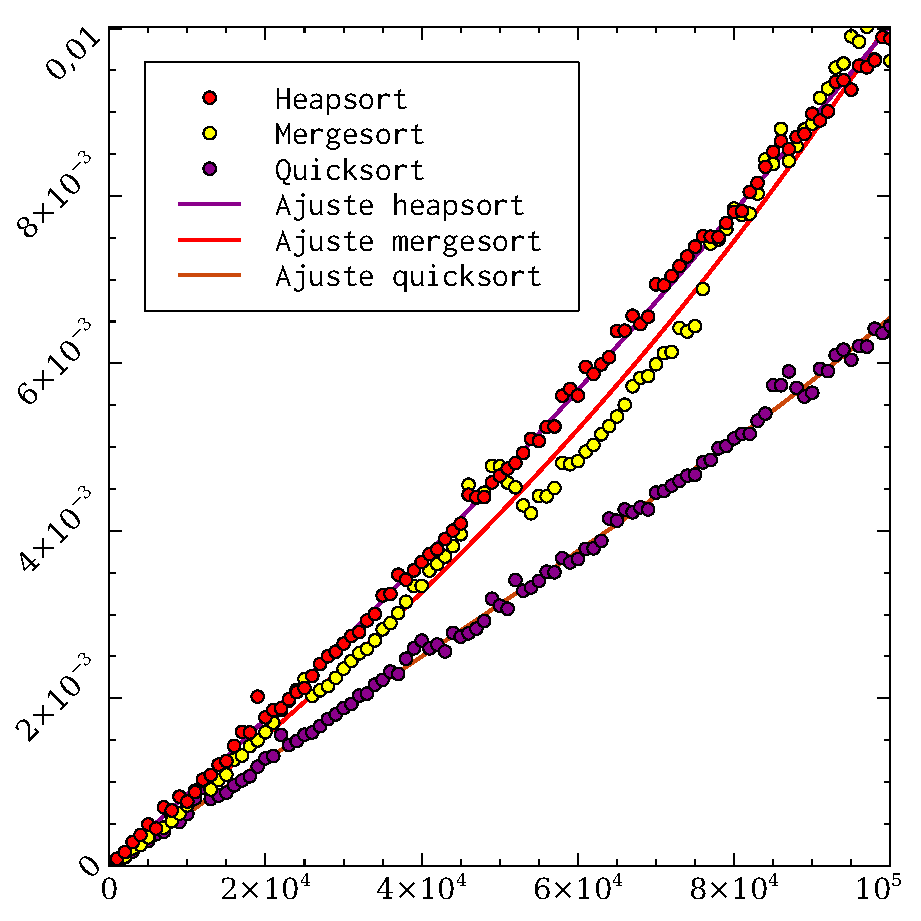
\includegraphics[]{nlogn_ajuste.eps}
%  \label{fig:ejemplo}
%\end{figure}
}
\end{center}
\end{frame}
\begin{frame}
\frametitle{Gráfica de algoritmos $O(n^2)$}
\begin{center}
\scalebox{0.53}[0.5]{
%	\begin{figure}
%  \centering
    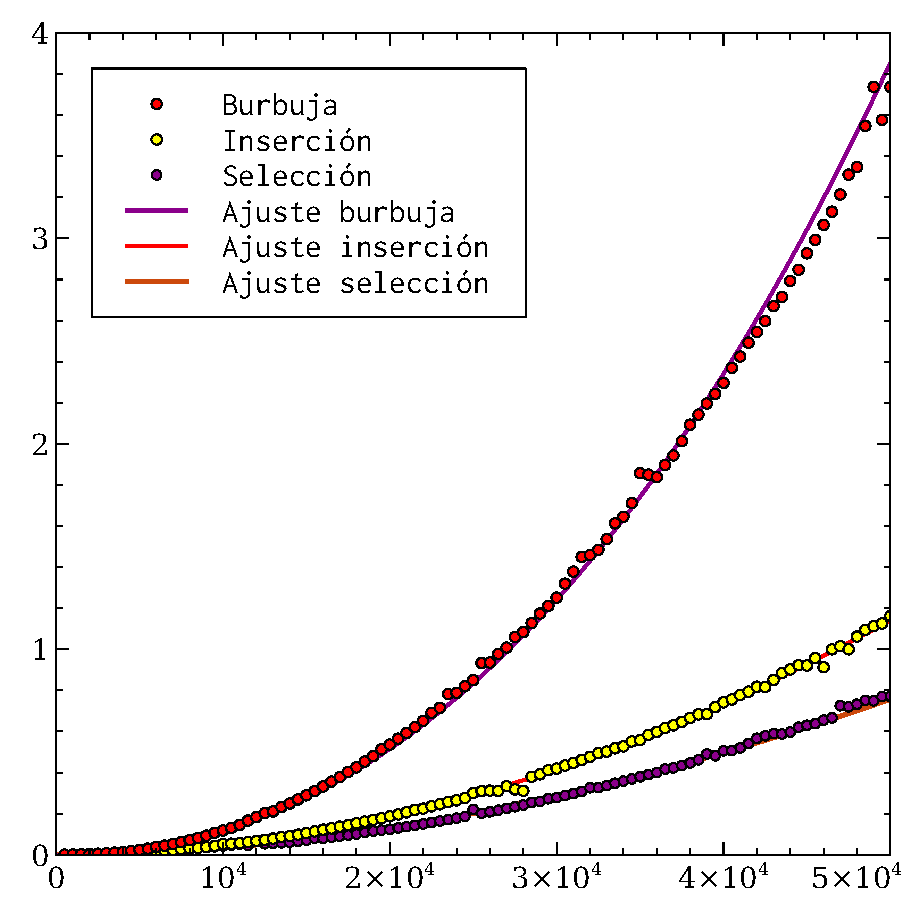
\includegraphics[]{n2_ajuste}
%  \label{fig:ejemplo}
%\end{figure}
}
\end{center}
\end{frame}
\begin{frame}
\frametitle{Gráfica del algoritmo $O(n^3)$}
	ESTA GRÁFICA NO COMPILA, AHORA LO ARREGLO
%	\begin{center}
%\scalebox{0.53}[0.5]{
%	\begin{figure}
%  \centering
 %   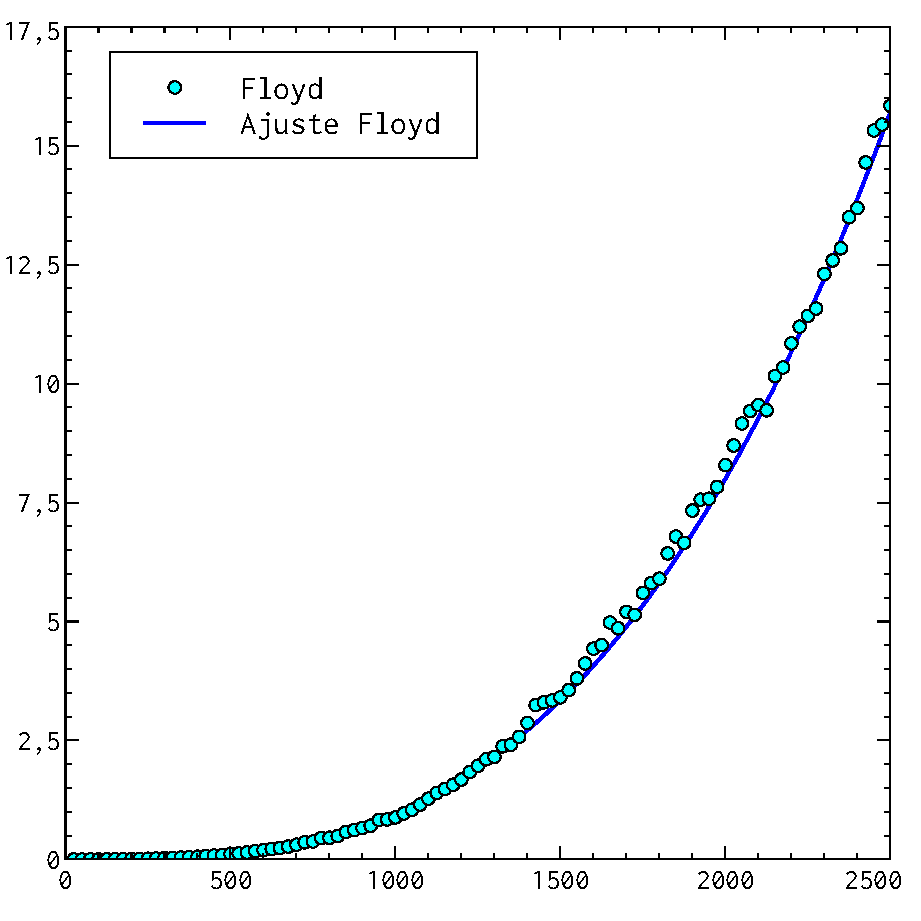
\includegraphics[]{n3_ajuste.eps}
%  \label{fig:ejemplo}
%\end{figure}
%}
	%\end{center}
\end{frame}
\begin{frame}
\frametitle{Gráfica del algoritmo $O(2^n)$}
	\begin{center}
\scalebox{0.53}[0.5]{
%	\begin{figure}
%  \centering
    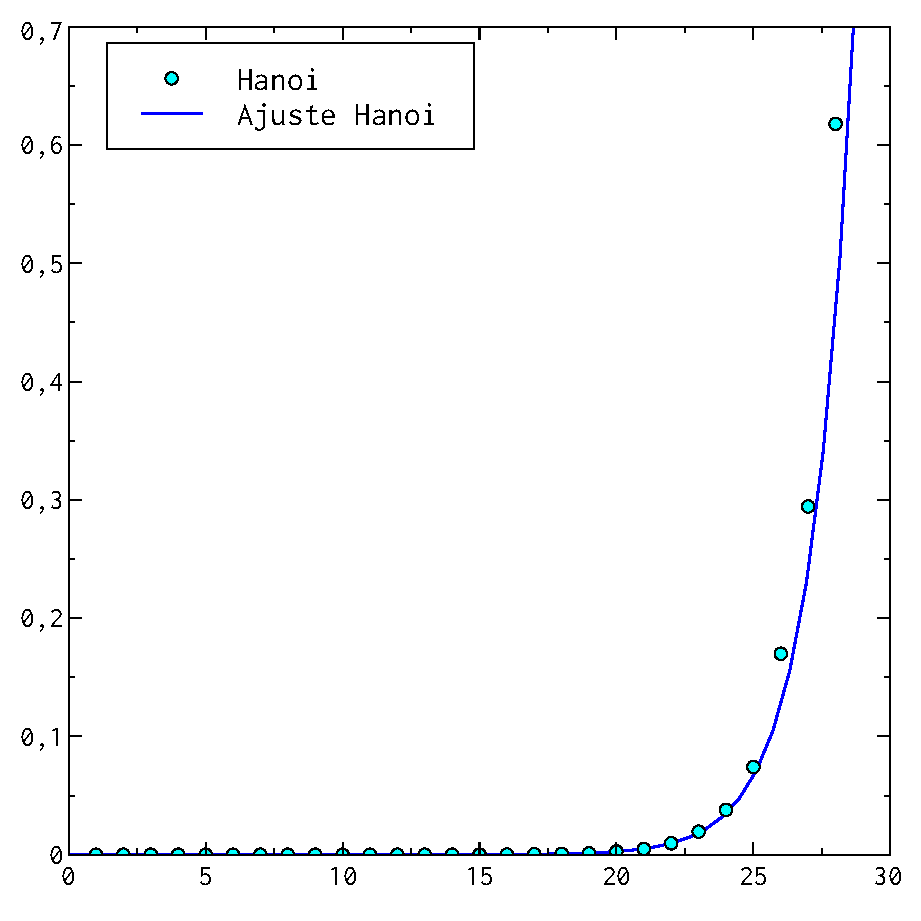
\includegraphics[]{2n_ajuste.eps}
%  \label{fig:ejemplo}
%\end{figure}
}
\end{center}
\end{frame}


\section{Ejercicio 2}
\subsection{Enunciado}

\begin{frame}
	2. Con cada una de las tablas anteriores, genere un gráfico comparando los tiempos  de
los algoritmos. Indique claramente el significado de cada serie. Para los algoritmos que
realizan la misma tarea (ordenar) exponga una tabla compartida dondea poder apreciar las diferencias en rendimiento de algoritmos con diferente orden de
eficiencia.
	\begin{figure}
  \centering
    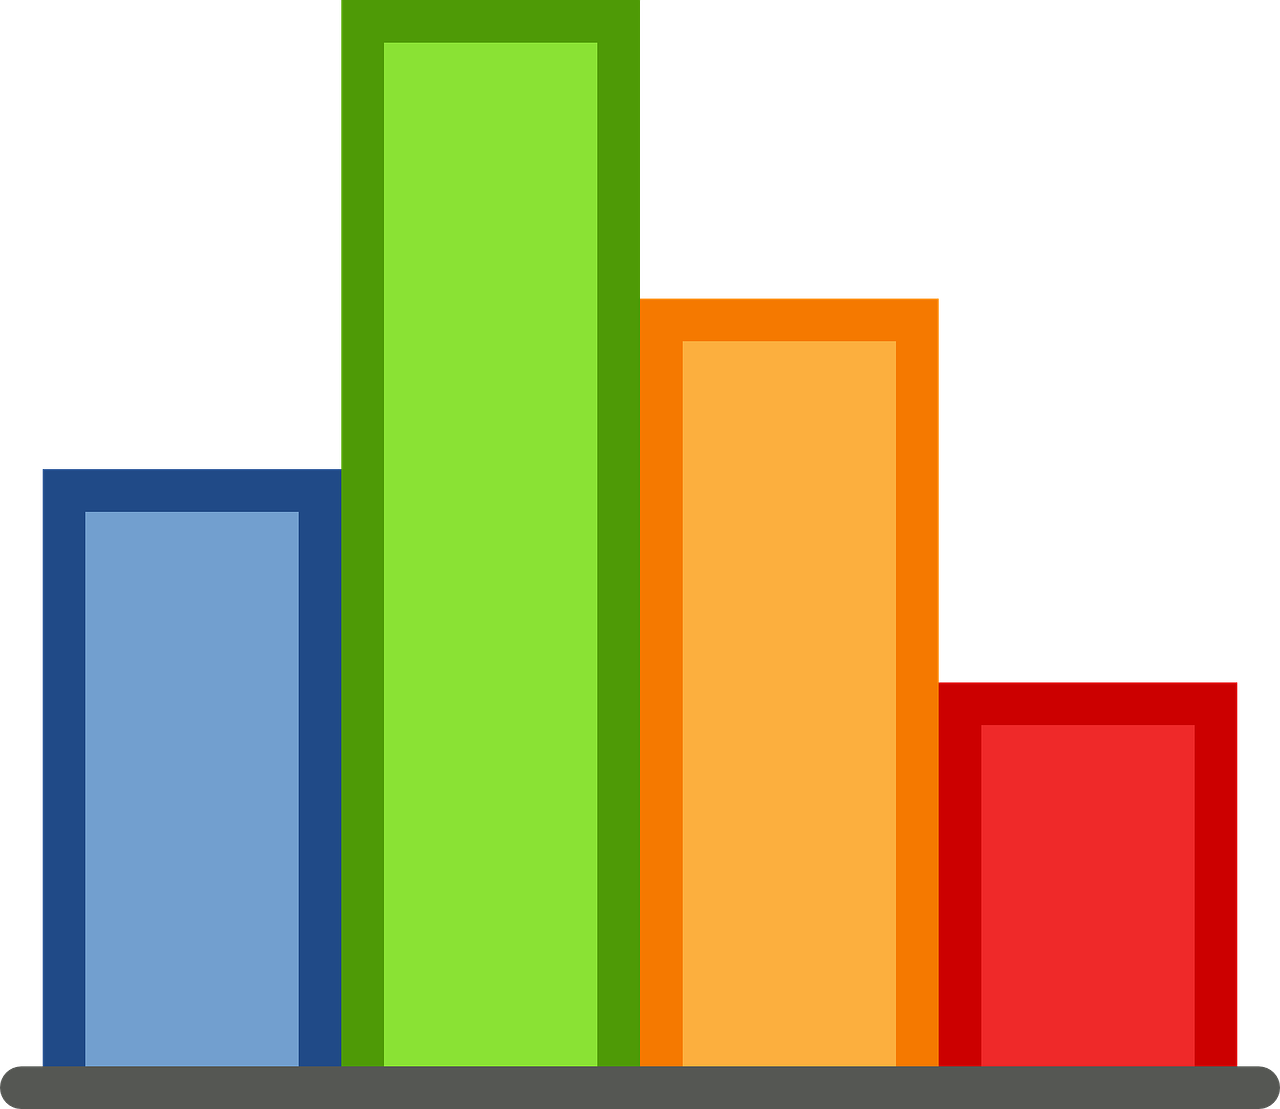
\includegraphics[width=0.3\textwidth]{graf.png}
  \label{fig:ejemplo}
\end{figure}
\end{frame}
\subsection{Solución}
\begin{frame}
Las gráficas por ordenes de eficiencia ya las mostramos en el ejercicio anterior. Ahora proseguiremos explicando como las generamos y exponiedo como las hallamos (uso de gnuplot)
\end{frame}
\begin{frame}
\frametitle{Comparación algoritmos ordenación}
	\begin{figure}
  \centering
    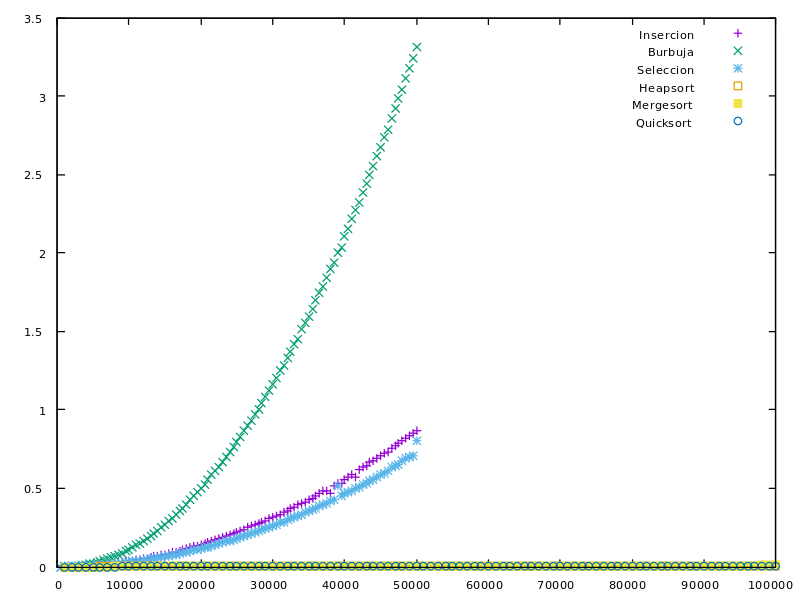
\includegraphics[width=0.98\textwidth]{Ordenacion.png}
  \label{fig:ejemplo}
\end{figure}
\end{frame}
\section{Ejercicio 3}
\subsection{Enunciado}
\begin{frame}
3. Calcule también la eficiencia híbrida de todos los algoritmos,  siguiendo las pautas inidcadas en la sección 4. Pruebe también con otros ajustes que no se correpondan con la eficiencia teórica (ajuste lineal, cuadrático, etc) y copruebe la variación en la calidad del ajuste.
\end{frame}
\subsection{Solución}
\frame{
	Esto es una explicación accesoria que quita seriedad, borradla si os parece oportuno.\\
	
	
	Para realizar la eficiencia teórica vamos a coger el analisis hecho en teoría y a ajustar las curva por mínimos cuadrados. Ahora expondremos los resultados de nuestro análisis.
}
\frame{
\frametitle{Coeficientes de los ajustes de las curvas $O(n\log n)$}
\begin{block}{Curva parametrizada}
	$ax\log(x)+bx$
\end{block}
}

\frame{
\frametitle{Coeficientes de los ajustes de las curvas $O(n\log n)$}
\resizebox{\textwidth}{!}{
\begin{tabular}{ll}
	Algoritmo & Coeficientes\\ \hline\noalign{\smallskip}
	\textit{Heapsort} & $\begin{array}{ll}
	a = 4,45661980236212e-9\\
b = 4,57091330896553e-8
\end{array}$ \\\hline\noalign{\smallskip}
	\textit{Mergesort} & $\begin{array}{ll}
	a = 1,04427553800116e-8\\
b = -2,58720994439492e-8
\end{array}$\\\hline\noalign{\smallskip}
	\textit{Quicksort} & $\begin{array}{ll}
	a = 2,79493370281663e-9\\
b = 3,29731080614046e-8
\end{array}$\\ \hline\noalign{\smallskip}
	
\end{tabular}
}
}

\frame{
\frametitle{Coeficientes de los ajustes de las curvas $O\left(n^2\right)$}
\begin{block}{Curva parametrizada}
	$a+bx+cx^2$
\end{block}


}

\frame{
\frametitle{Coeficientes de los ajustes de las curvas $O\left(n^2\right)$}
\begin{center}
\begin{tabular}{ll}
Algoritmo & Coeficientes\\ \hline\noalign{\smallskip}
Burbuja  &  $\begin{array}{lll}
	a = 0,00082695543722856\\
b = -1,78008100621617e-6\\
c = 1,41949043281942e-9
\end{array}$  \\\hline\noalign{\smallskip}
	Inserción  & $\begin{array}{lll}
	a = 9,34565785754161e-6\\
b = 4,03176585100252e-8\\
c = 4,60339062991612e-10
\end{array}$\\\hline\noalign{\smallskip}
	Selección  & $\begin{array}{lll}
	a = -3,46794858274209e-5\\
b = 1,18720037408458e-7\\
c = 3,13826775410318e-10
\end{array}$\\
\end{tabular}
\end{center}
}
\frame{
\frametitle{Coeficientes de los ajustes de la curva $O\left(n^3\right)$ (Floyd)}
\begin{block}{Curva parametrizada}
	$a+bx+cx^2+dx^3$
\end{block}
}

\frame{
\frametitle{Coeficientes de los ajustes de la curva $O\left(n^3\right)$ (Floyd)}
\begin{center}
\begin{tabular}{ll}
Algoritmo & Coeficientes\\ \hline\noalign{\smallskip}
Floyd  & $\begin{array}{llll}
	a = -0,0001373576928425\\
b = 7,19449328754654e-6\\
c = -6,0356967827879e-8\\
d = 1,02809541531643e-9
\end{array}$\\
\end{tabular}
\end{center}
}

\frame{
\frametitle{Coeficientes de los ajustes de la curva $O\left(2^n\right)$ (Hanoi)}
\begin{block}{Curva parametrizada}
	$a2^{bx}$
\end{block}
}

\frame{
\frametitle{Coeficientes de los ajustes de la curva $O\left(2^n\right)$ (Hanoi)}
\begin{center}
\begin{tabular}{ll}
Algoritmo & Coeficientes\\ \hline\noalign{\smallskip}
Hanoi  & $\begin{array}{ll}
	a = 7,0670287742651e-9\\
b = 0,92649353651508
\end{array}$
\end{tabular}
\end{center}
}
\section{Ejercicio 4}
\subsection{Enunciado}
\frame{Otro aspecto interesante a analizar mediante este tipo de estudio es la variación de la eficiencia empírica en función de parámetros externs tales como: las opciones de compilación utilizada (con/sin optimización), el ordenador donde se realizan las pruebas, el sistea operativo, etc. Sugiera algún estudio de este tipo,consulte con el profesor de prácticas y llevelo a cabo.} 
\subsection{solución}
\end{document}
